\mychapter{Còniques i llocs geomètrics}{Còniques i llocs geomètrics}{
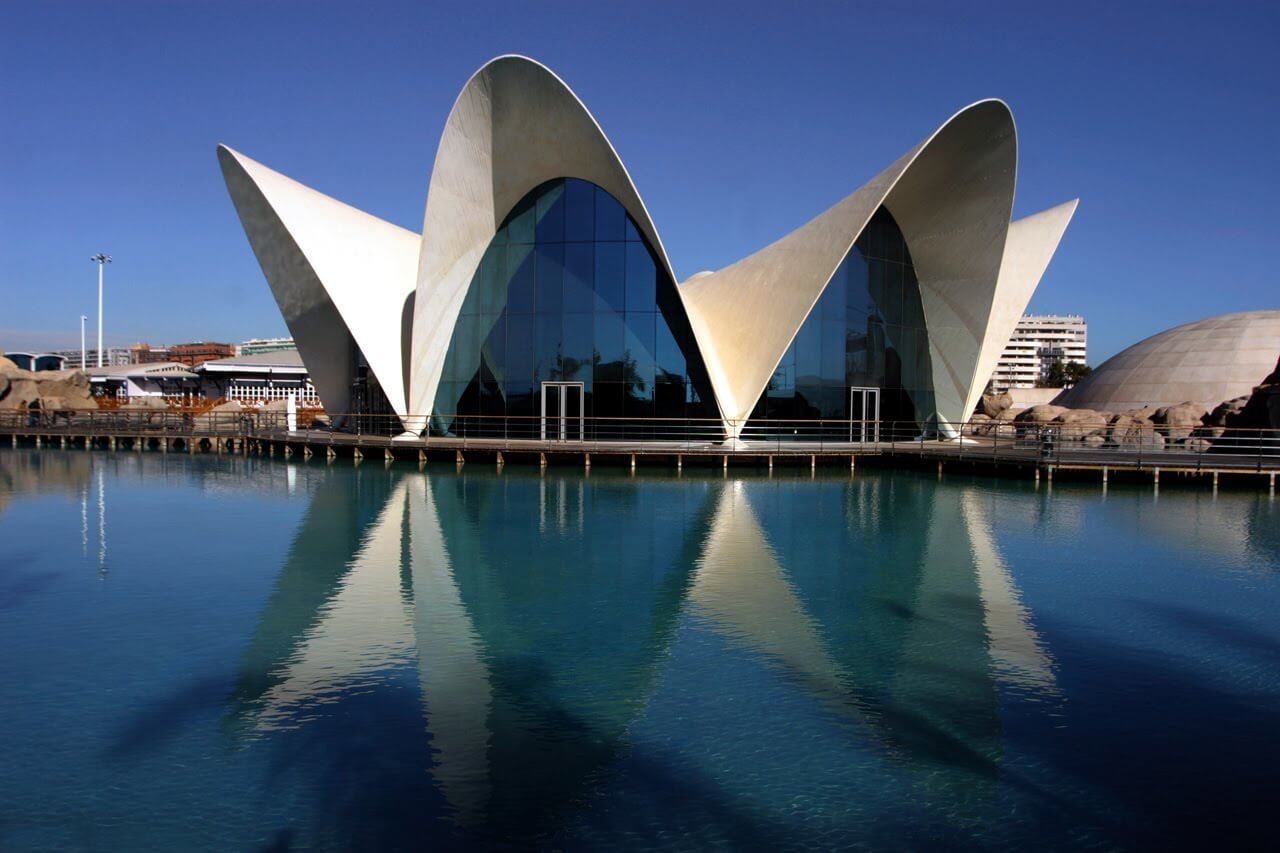
\includegraphics[width=4.5cm]{img-10/conicas}
}{chap:coniques}

\section{Concepte de lloc geomètric}
\begin{theorybox}
	Un lloc geomètric és un conjunt de punts $(x,y)$ del pla que compleixen una certa condició. 
	
	Per exemple, el conjunt  $\{ (x,y) \,\, \text{tals que } y=x \}$ és una forma d'expressar tots els punts que es troben sobre la recta $y=x$.
	
	La bisectriu de costats les rectes $r_1$, $r_2$ és el lloc geomètric  
	\begin{equation*}
	\{X(x,y) \,\, \text{tals que } dist(X,r_1)=dist(X,r_2)\}  
	\end{equation*}
	
	Una circumferència de centre $O$ i radi $R$ són tots els punts de
	\begin{equation*}
	  \{X(x,y) \,\, \text{tals que } dist(X,O)=R\}
	\end{equation*}
\end{theorybox}

\begin{mylist}
	\item Troba el lloc geomètric dels punts que equidisten de $A(5,-3)$  i $B(2,0)$.
	
	\answers{$d(A,X)=d(B,X)$.\par $(x-5)^2+(y+3)^2=(x-2)^2+y^2$\par $y=x-5$ és la mediatriu del segment AB}
	
	\item Calcula el lloc geomètric dels punts $(x,y)$ tals que la diferència dels quadrats de les distàncies als punts $A(0,0)$ i $B(6,3)$ sigui igual a 15. Quina figura obtens?
	
	\answers{$d^2(X,A)-d^2(X,B)=15$.\par $x^2+y^2 - \left( (x-6)^2+(y-3)^2 \right)=15$. És la recta $y=-2x+10$.}
	
	\item Troba tots els punts del pla que equidisten de les rectes
	\begin{equation*}
	r: \, 4x-3y+8=0 \,\,\, \text{i}\,\,\, s:\, 12x+5y-7=0
	\end{equation*}

	\answers{$d(X,r)=d(X,s)$.\par $\dfrac{|4x-3y+8|}{5}=\dfrac{|12x+5y-7|}{13}$, dóna dues equacions 
	$13(4x-3y+8)=\pm 5(12x+5y-7)$\par Per cadascun dels signes, trobam una rectes com a lloc geomètric: $8x+64y-139=0$ i $112x-14y+69=0$\par
	Corresponen a les dues bisectrius de les dues rectes. \par
	\ggblink{https://www.geogebra.org/m/vpkYZGqu}
}
\end{mylist}

\pagebreak
\section{Les còniques com a seccions d'una superfície cònica}
\begin{theorybox}
\begin{multicols}{4}
	\scriptsize
	Si el pla que talla a la superfície cònica és perpendicular a l'eix, la secció és una \textbf{circumferència}.
		\begin{center}
	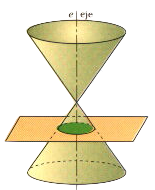
\includegraphics[height=3.cm]{img-10/circumferencia.png}
	\end{center}

	Si inclinam el pla de manera que sigui oblic amb l'eix i talli a totes les generatrius, la secció és una \textbf{el·lipse}.
		\begin{center}
		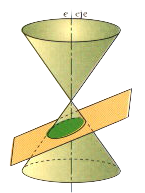
\includegraphics[height=3.cm]{img-10/ellipse.png}
	\end{center}

	Si continuam inclinant el pla de manera que sigui paral·lel a una generatriu, resulta una \textbf{paràbola}.
		\begin{center}
		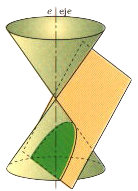
\includegraphics[height=3.cm]{img-10/parabola.png}
\end{center}
		
	Finalment, si inclinam encara més el pla, obtenim una figura amb dues branques que s'anomena \textbf{hipèrbola}.
		\begin{center}
		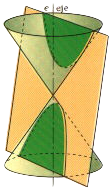
\includegraphics[height=3.cm]{img-10/hiperbola.png}
	\end{center}

\end{multicols}	
\end{theorybox}



%%%%%%%%%%%%%%%%%%%%%%%%%%%%%%%%%%%%%%%%%%%%%%%%%%%%%%%%%%%%%%%%%%%%%%%%%%%%%%%%%%%%%%%%%%%%%%%%%%%%%%%%%%%%%%%%%%%%%%%%%%%%%%%

\section{La circumferència}

\begin{theorybox}
	\videonw{194}{La circumferència}
	\begin{wrapfigure}{R}{0.3\textwidth} 
		\vspace{-0.5cm}
		\begin{center}
			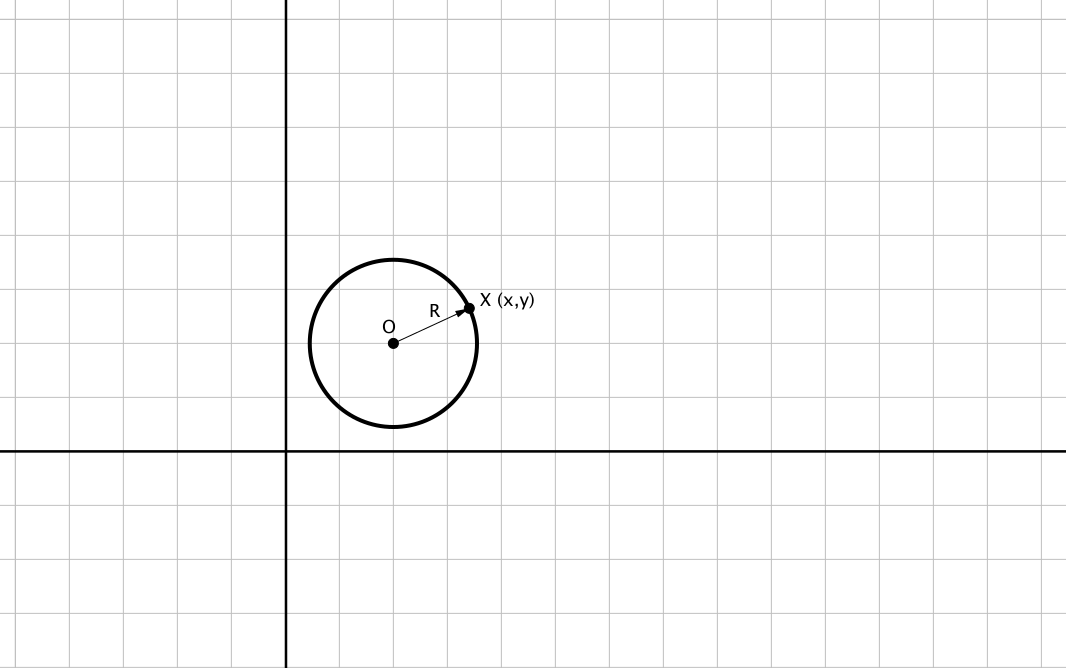
\includegraphics[width=0.26\textwidth]{img-10/circ2}
			\end{center}
	 \end{wrapfigure}
	\textbf{És defineix una circumferència com el lloc geomètric de tots els punts del pla
	que equidisten d'un punt anomenat centre.}
	
	L'equació canònica d'una circumferència de radi $R$ i centre el punt $O(x_0, y_0)$ és:
	\begin{equation}
		\label{eq:circ-canonica}
		(x-x_0)^2+(y-y_0)^2=R^2
	\end{equation}
	
	Si efectuam els quadrats en l'equació (\ref{eq:circ-canonica}) obtindrem l'expressió general de la circumferència:
	\begin{equation}
		\label{eq:circ-genreal}
		x^2+y^2+Ax+By+C=0
	\end{equation}
	essent $A=-2x_0$, $B=-2y_0$, $C=x_0^2+y_0^2-R^2$. És important notar que només serà possible formar una circumferència si $x_0^2+y_0^2-C > 0$.
	
\end{theorybox}

\begin{resolt}[Exemple]{Calcula l'equació canònica i general de la circumferència de centre $O(3,0)$ i que passa pel punt $P(5,2)$.}
	 En primer lloc calculam el radi 
	 
	 \[R=dist(O, P)=\sqrt{(5-3)^2+(2-0)^2}=\sqrt{8}\]
	 
	 L'equació canònica és $(x-3)^2+(y-0)^2=8$. Si efectuam els quadrats, trobam l'equació general: $x^2+y^2-6x+1=0$. 
\end{resolt}
\pagebreak
\begin{resolt}{Donada la circumferència d'equació 
		
		$x^2+y^2+4x-10y+13=0$ 
		
		troba el seu centre i radi.}
	 De l'equació general identificam els coeficients $A=4$, $B=-10$ i $C=13$. Si utilitzam les relacions:  $4=-2x_0$,  $-10=-2y_0$ automàticament tenim el centre $x_0=-2$ i $y_0=5$. 
	 
	 Per trobar el radi utilitzam la darrera relació: $13=(-2)^2+5^2-R^2$. Si d'aquí aïllam $R$ trobam $R=4$.
	 
	  Aquesta circumferència té d'equació canònica $(x+2)^2+(y-5)^2=4^2$.	
\end{resolt}

\begin{mylist}

	\exer[1]  Calcula l'equació de la circumferència que passa pel punt $A=(1, 1)$ i té per centre a  $O=(-1, 3)$.
	\answers{Radi $\sqrt{8}$, $(x+1)^2+(y-3)^2=8$}
	
    \exer[1]  Comprova que $x^{2} -2x+y^{2} =0$ és l'equació d'una circumferència. Troba'n el centre i el radi. Dibuixa-la.
	 \answers{Centre $O(1,0)$, radi $R=1$}
	 
\end{mylist}

%%%%%%%%%%%%%%%%%%%%%%%%%%%%%%%%%%%%%%%%%%%%%%%%%%%%%%%%%%%%%%%%%%%%%%%%%%%%%%%%%%%%%%%%%%%%%%%%%%%%%%%%%%%%%%%%%%%%%%%%%%%%%%%
\section{L'el·lipse}
\begin{theorybox}
	\videonw{195}{L'el·lipse}
	\textbf{És defineix l'el·lipse com el lloc geomètric de tots els punts del pla
    tals que la \textit{suma de les distàncies} a dos punts fixos anomenats focus es manté constant.}
	
	L'equació canònica d'una el·lipse de semieixos $a$ i $b$ i centre el punt $O(x_0, y_0)$ és:
	\begin{wrapfigure}{R}{0.3\textwidth} 
		\vspace{-1cm}
		\begin{center}
			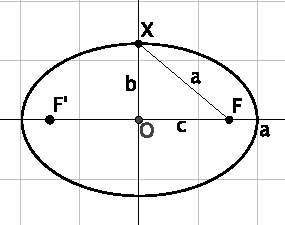
\includegraphics[width=0.28\textwidth]{img-10/ellip2}
		\end{center}
		\vspace{-1cm}
	\end{wrapfigure}
	\begin{equation}
	\label{eq:ellipse-canonica}
	\frac{(x-x_0)^2}{a^2}+\frac{(y-y_0)^2}{b^2}=1
	\end{equation}
	
	
	Quan els semieixos d'una el·lipse són iguals $a=b=R$, trobam l'equació (\ref{eq:circ-canonica}) de la circumferència.
	
	Els vèrtexs estan situats en els punts $(x_0-a, y_0)$, $(x_0+a, y_0)$, $(x_0, y_0-b)$, $(x_0, y_0+b)$. Els focus els trobam en els punts $F(x_0+c, y_0)$ i $F'(x_0-c,y_0)$.
	
	Definim $c$ com la semi-distància focal. A qualsevol el·lipse \fbox{$a^2=b^2+c^2$}. 
	
	Una mesura de quan estirada és una el·lipse ens ho dóna l'excentricitat $e=\frac{c}{a}$. Per una el·lipse es compleix que $0<e<1$. Quan $e \rightarrow 0$ és pràcticament una circumferència i $e \rightarrow 1$ s'assembla a un ``espagueti''. 
	
\end{theorybox}


\begin{resolt}[E]{Calcula l'equació de l'el·lipse sabent que té centre a $O(0,0)$, té semieix major 8 i que un dels focus és al punt $F(3,0)$. Calcula la seva excentricitat. }
	Si el centre és $(0,0)$, l'equació canònica es redueix a $\frac{x^2}{a^2}+\frac{y^2}{b^2}=1$. Una de les dades és que el semieix major val $a=8$ i que la semi-distància focal és $c=3$. Falta trobar $b=\sqrt{a^2-c^2}=\sqrt{55}$. L'equació és: $\frac{x^2}{64}+\frac{y^2}{55}=1$.
	
	L'excentricitat és $e=c/a = 3/8 = 0.375 $, òbviament menor que 1.
	
\end{resolt}
\begin{resolt}{Donada l'equació de l'el·lipse  $\frac{x^2}{9}+y^2=1$, troba la posició dels seus focus i dels vèrtexs. Troba la seva excentricitat. }
 
	
	En primer lloc veim que el centre és el punt $(0,0)$. El semieix major val $a=\sqrt{9}=3$ i el semi-eix menor $b=1$. La semi-distància focal es troba de $c=\sqrt{a^2-b^2}=\sqrt{8}$. 
	\vspace{0.25cm}
	
	Els vèrtexs estan a $(-3,0)$; $(3,0)$; $(0,1)$; $(0,-1)$. Els dos focus es troben a $F'(-\sqrt{8},0)$ i $F(\sqrt{8},0)$.  
	\vspace{0.25cm}
	
	L'excentricitat és $e=c/a = \sqrt{8}/3 = 0.943$ propera a 1, cosa que ens indica que és bastant allargada.
	
\end{resolt}

\begin{mylist}
	
	\exer[1] Calcula el centre, semi-eixos, focus i excentricitat de l'el·lipse \linebreak  $\frac{\left(x+1\right)^{2} }{9} +\frac{\left(y-1\right)^{2} }{4} =1$.
	\answers{Centre $O(-1,1)$, semi-eixos $a=3$, $b=2$, focus $F'(-1-\sqrt{5}, 1)$ i $F'(-1+\sqrt{5}, 1)$. Excentricitat $e=0.745$}
	
	\exer[1] Una el·lipse té focus en $(-2, 0)$ i en $(2, 0)$ i passa pel punt $(3, 0)$. Calcula la seva equació i dibuixa-la. Quant val l'excentricitat?
	\answers{$\frac{x^2}{9}+\frac{y^2}{5}=1$ $e=2/3$}
	
	\exer[1] Calcula l'equació d'una el·lipse centrada a l'origen en vèrtex en el punt $V(10,0)$ i excentricitat $e=0.2$.
	\answers{$\frac{x^2}{100}+\frac{y^2}{96}=1$}
	
\end{mylist}

%%%%%%%%%%%%%%%%%%%%%%%%%%%%%%%%%%%%%%%%%%%%%%%%%%%%%%%%%%%%%%%%%%%%%%%%%%%%%%%%%%%%%%%%%%%%%%%%%%%%%%%%%%%%%%%%%%%%%%%%%%%%%%%
\section{La hipèrbola}
\begin{theorybox}
	\videonw{196}{La hipèrbola}
	\textbf{És defineix la hipèrbola com el lloc geomètric de tots els punts del pla
	tals que la \textit{diferència de les distàncies} a dos punts fixos anomenats focus es manté constant.}
	
	L'equació canònica d'una hipèrbola de semieixos $a$ i $b$ i centre el punt $(x_0, y_0)$ és:
		\begin{wrapfigure}{R}{0.34\textwidth} 
		\vspace{-1cm}
		\begin{center}
			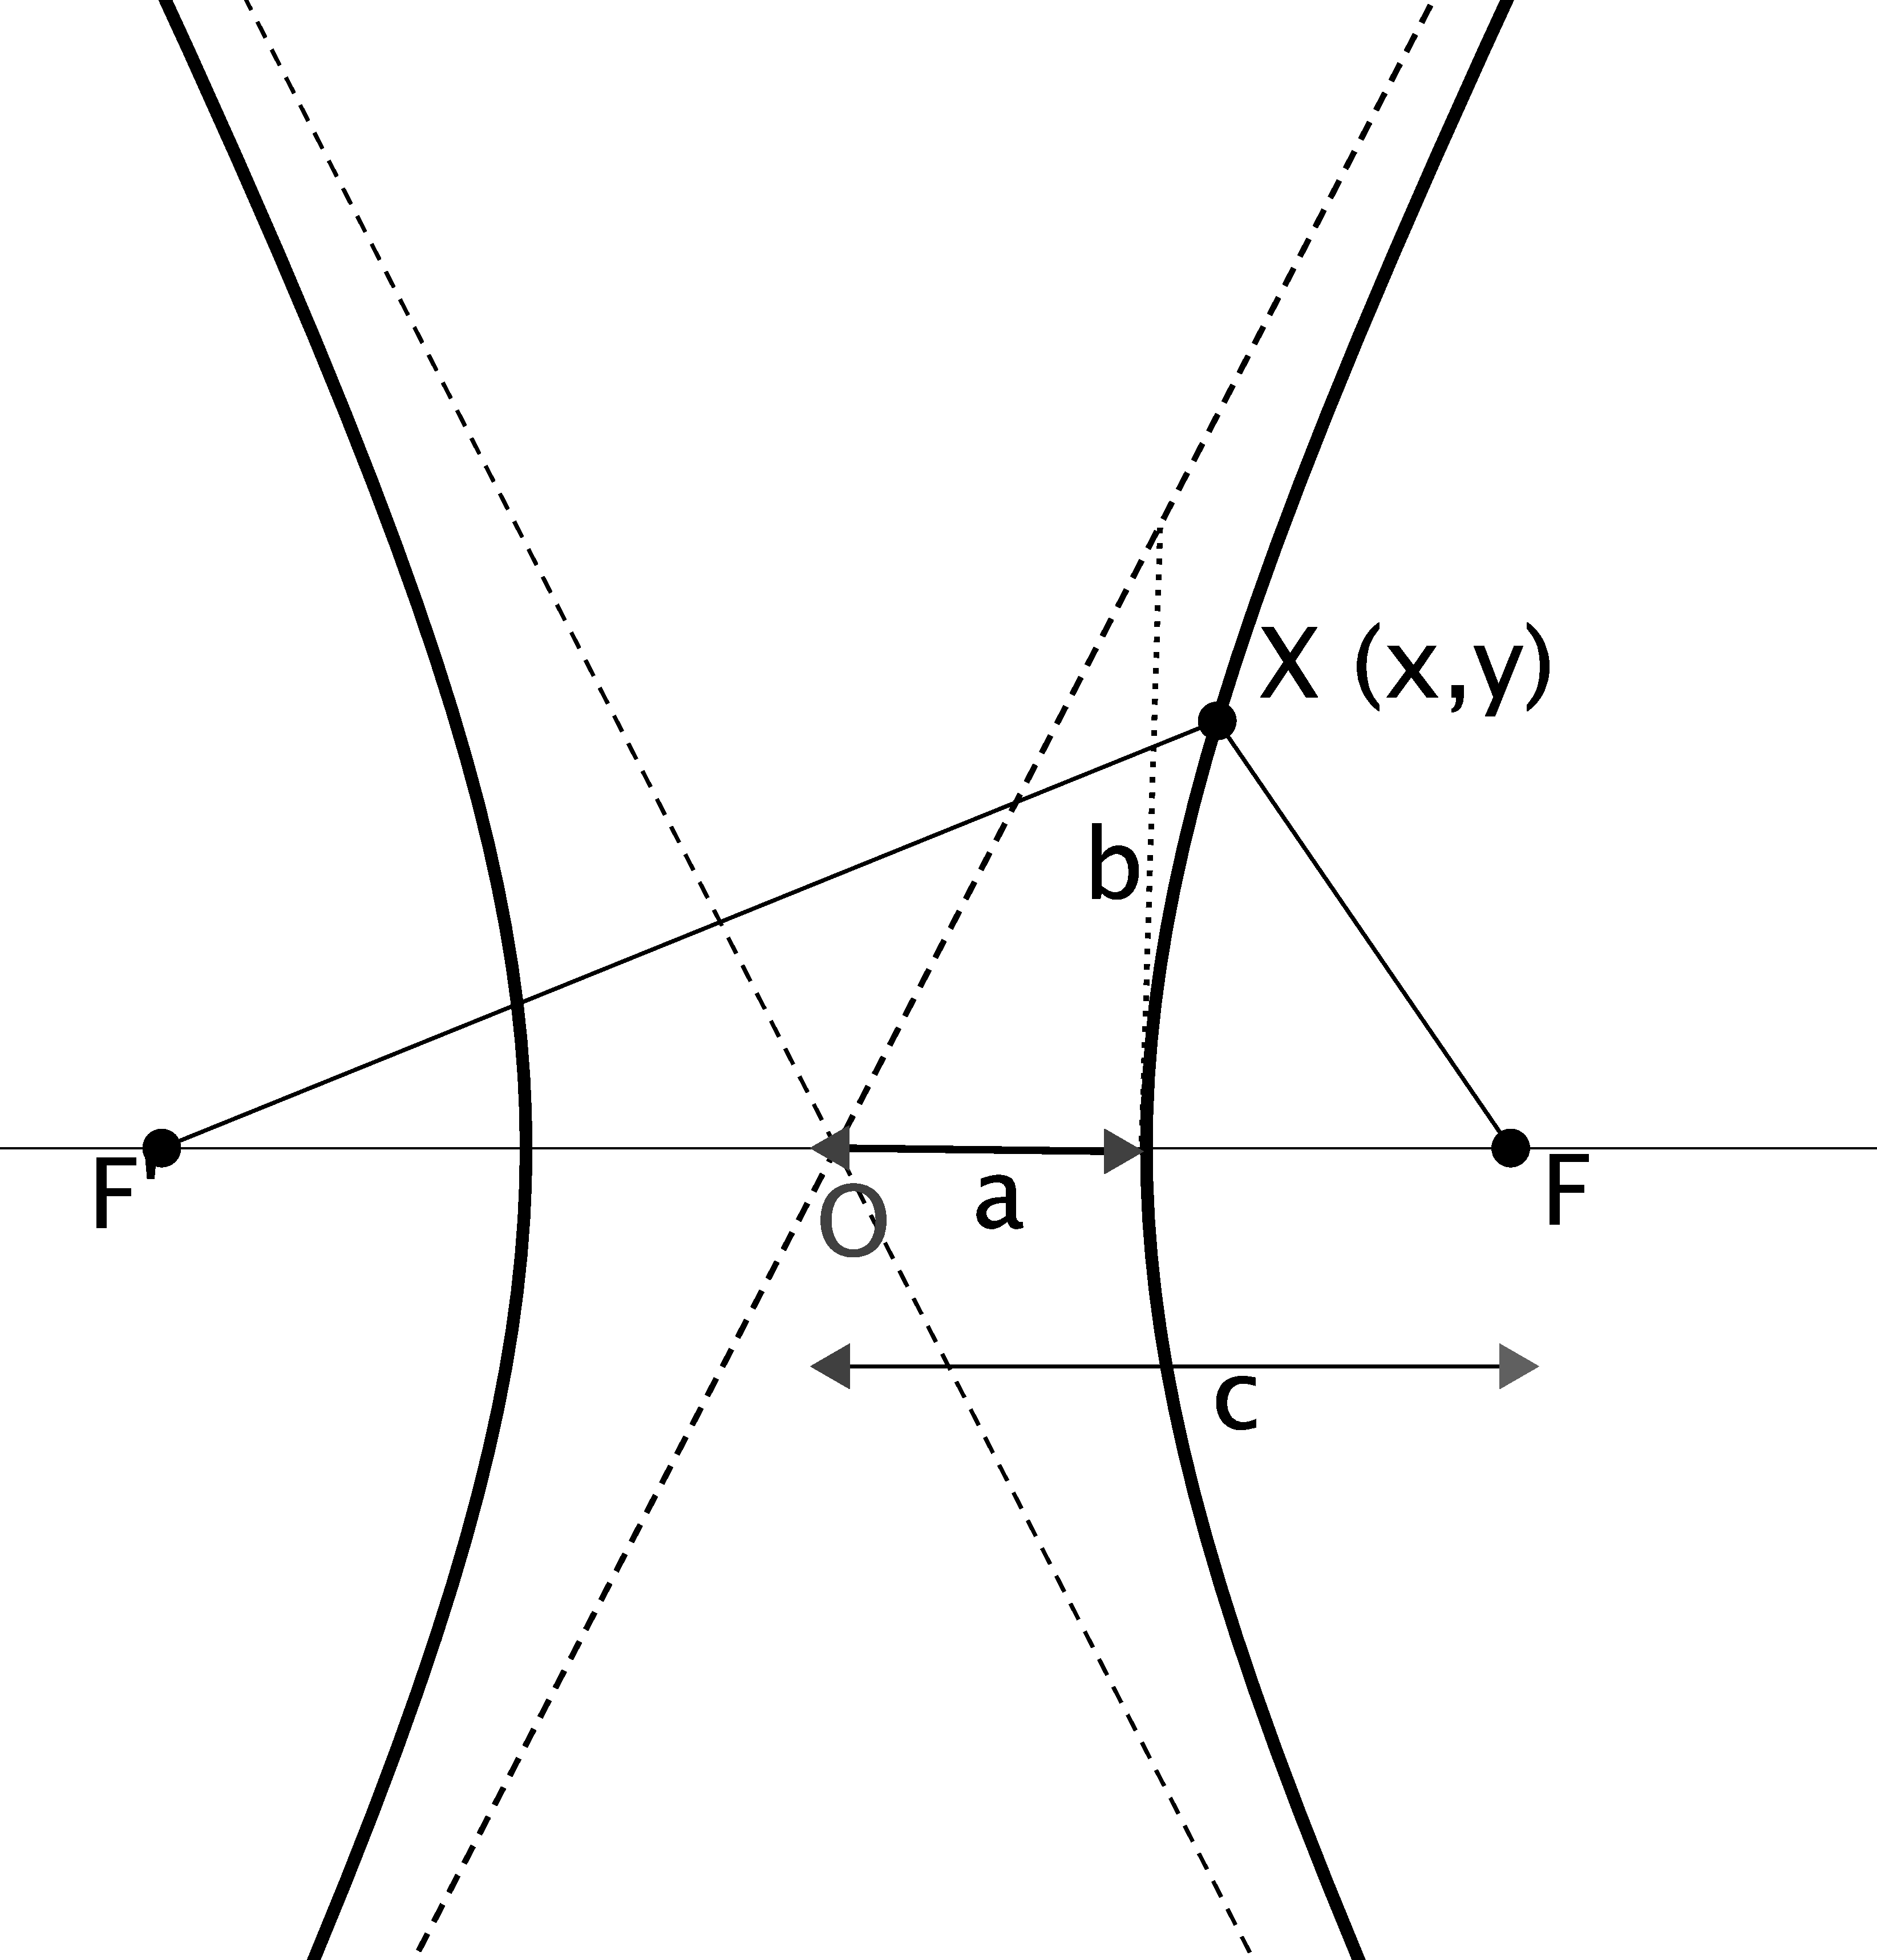
\includegraphics[width=0.32\textwidth]{img-10/hiperb2}
		\end{center}
			\vspace{-1cm}
	\end{wrapfigure}
	\begin{equation}
	\label{eq:hiperbola-canonica}
	\frac{(x-x_0)^2}{a^2}-\frac{(y-y_0)^2}{b^2}=1
	\end{equation} 
	
	Els vèrtexs estan situats en els punts $(x_0-a, y_0)$, $(x_0+a, y_0)$. Els focus els trobam en els punts $F(x_0+c, y_0)$ i $F'(x_0-c,y_0)$.
	
	Definim $c$ com la semi-distància focal. A qualsevol hipèrbola es compleix que  \fbox{$c^2=a^2+b^2$}. L'excentricitat $e=\frac{c}{a}$ per una hipèrbola compleix que $e>1$. 
	
	
	
	Les dues branques d'una hipèrbola s'acosten a dues asímptotes obliqües que tenen com equacions \newline $y-y_0=\pm \frac{b}{a} (x-x_0)$. 
	
	Si $a=b$, es diu \textbf{hipèrbola equilàtera} i es compleix que les dues asímptotes formen un angle recte. Si prenem les asímptotes com a eixos, l'equació de la hipèrbola equilàtera es trasforma en $xy=k$.
\end{theorybox}
\pagebreak

\begin{resolt}[E]{Calcula l'equació de la hipèrbola sabent que té centre a $O(0,0)$, semi-distància focal 6 i excentricitat 2. Calcula les seves asímptotes. Representa-ho tot gràficament.}
  	\begin{wrapfigure}{R}{0.34\textwidth} 
		\vspace{-0.5cm}
		\begin{center}
			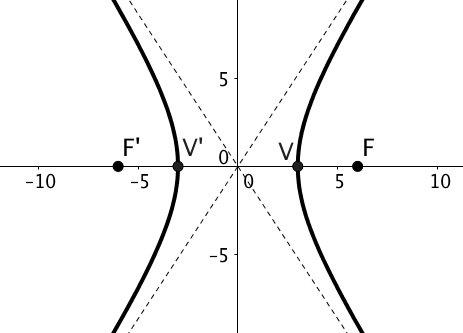
\includegraphics[width=0.3\textwidth]{img-10/exem-h2.png}
		\end{center}
	\end{wrapfigure}

	Si el centre és $(0,0)$, l'equació canònica es redueix a \linebreak $\frac{x^2}{a^2}-\frac{y^2}{b^2}=1$. Una de les dades és que el semi-distància focal val $c=6$ i que l'excentricitat és $e=2$. Sabem que $e=c/a$, i d'aquí aïllam el semieix major  $a=c/e=6/2=3$. Falta trobar el semi-eix menor $b=\sqrt{c^2-a^2}=\sqrt{27}$. L'equació és: $\frac{x^2}{9}-\frac{y^2}{27}=1$.
	
	Les asímptotes són $y=\pm \frac{\sqrt{27}}{6}x$.
\end{resolt}
\begin{resolt}{ Donada l'equació de la hipèrbola  $x^2-y^2=9$, troba la posició dels seus focus i dels vèrtexs. Calcula la seva excentricitat. }
  
	Es tracta d'una hipèrbola equilàtera $a=b=3$. El centre és el punt $(0,0)$. La semi-distància focal es troba de $c=\sqrt{a^2+b^2}=\sqrt{18}=3\sqrt{2}$. 
	
	Els vèrtexs estan a $(-3,0)$; $(3,0)$. Els dos focus es troben a $F'(-3\sqrt{2},0)$ i $F(3\sqrt{2},0)$.  
	
	L'excentricitat és $e=c/a = 3\sqrt{2}/3 = \sqrt{2}\approx 1.41$.
\end{resolt}

\begin{mylist}
\exer[1] Donada la hipèrbola $\dfrac{\left(x-1\right)^{2}}{16} -\dfrac{{y}^{2}}{9} =1$, calcula el centre, els seus focus, asímptotes i la seva excentricitat.
\answers{$O(1,0)$, $a=4$, $b=3$, $F'(-4,0)$ i $F(6,0)$, asímptotes $y=\pm 3(x-1)/4$, $e=5/4$.}
	
\exer[1]  Calcula l'equació de la hipèrbola equilàtera que té per focus $\left(2,\; 2\right)$ i $\left(-2,\quad 2\right)$, així com els seus paràmetres \textit{a}  i  \textit{b} i la seva excentricitat. Dibuixa-la.
\answers{$a=b=1/\sqrt{2}$, $2{x^2}-2(y-2)^2=1$, $e=\sqrt{2}$.}

\end{mylist}
 
%%%%%%%%%%%%%%%%%%%%%%%%%%%%%%%%%%%%%%%%%%%%%%%%%%%%%%%%%%%%%%%%%%%%%%%%%%%%%%%%%%%%%%%%%%%%%%%%%%%%%%%%%%%%%%%%%%%%%%%%%%%%%%%
\section{La paràbola}

\begin{theorybox}
	\videonw{197}{La paràbola}
	 \begin{wrapfigure}{R}{0.3\textwidth} 
		\vspace{-0.5cm}
		\begin{center}
			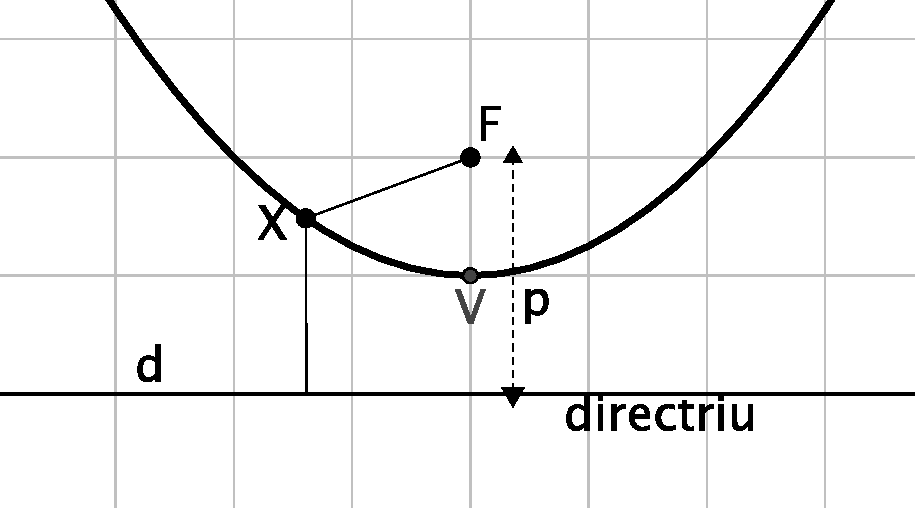
\includegraphics[width=0.28\textwidth]{img-10/parab2}
			\vspace{-1cm}
		\end{center}
	\end{wrapfigure}
	\textbf{És defineix la paràbola com el lloc geomètric de tots els punts del pla
	tals que la distància a un punt fix anomenat \textit{focus} és igual a la distància a una recta anomenada \textit{directriu}}.
	
	Si anomenam $p$ la distància entre el Focus i la directriu, i suposam que la directriu és la recta horitzontal $y=-p/2$ i el focus és al punt $F(0, p/2)$, trobam la paràbola vertical:
	 \begin{equation}
	\label{eq:parabola-v}
	y=\frac{1}{2p}x^2
	\end{equation} 
	Aquesta paràbola té el vèrtex en $V(0,0)$. Si desplaçam el vèrtex al punt $V(x_0,y_0)$, l'equació canviaria a $y-y_0=\dfrac{1}{2p}(x-x_0)^2$.
	
	Si la directriu és la recta horitzontal $x=-p/2$ i el focus és al punt $F(p/2, 0)$, trobam la paràbola horitzontal:
	\begin{equation}
	\label{eq:parabola-h}
	x = \frac{1}{2p}y^2
	\end{equation} 
	Aquesta paràbola també té el vèrtex en $V(0,0)$.
	 
 	Totes les paràboles tenen excentricitat $e=1$.
	 
\end{theorybox}


\begin{resolt}[E]{ Calcula l'equació de la paràbola que té el focus al punt $F(5,0)$ i com directriu la recta $x=-5$. Representa-la gràficament.
	}
	\begin{wrapfigure}{R}{0.3\textwidth} 
		\vspace{-0.5cm}
		\begin{center}
			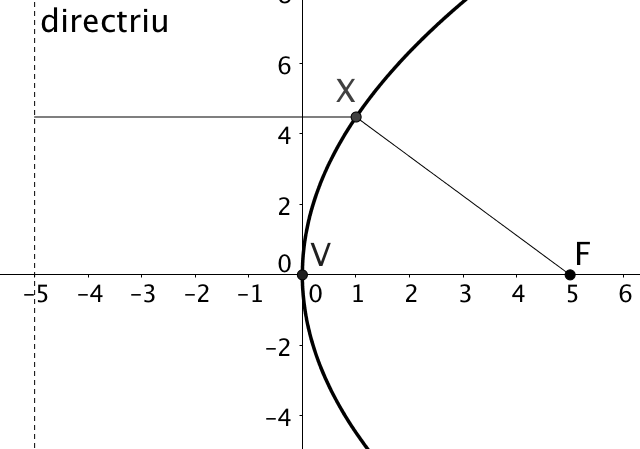
\includegraphics[width=0.28\textwidth]{img-10/exem-p1.png}
		\end{center}
	\end{wrapfigure}
	
	
	
	Es tracta d'una paràbola horitzontal amb $p=10$. El vèrtex és el punt $(0,0)$.  L'equació és $x=\frac{1}{20}y^2$.
	
	\vspace*{1.5cm}
	
\end{resolt}
\begin{resolt}{Considera la paràbola  $y=-2 x^2 + 1$, troba la posició del seu focus, el vèrtex i l'equació de la directriu. Representa gràficament la situació.}
	 \begin{wrapfigure}{R}{0.3\textwidth} 
		\vspace{-0.5cm}
		\begin{center}
			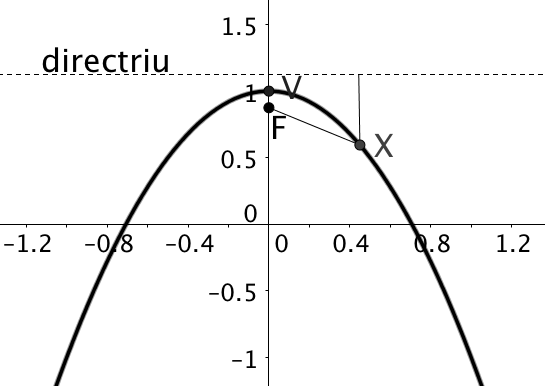
\includegraphics[width=0.28\textwidth]{img-10/exem-p2.png}
		\end{center}
	\end{wrapfigure}
 
	
	Es tracta d'una paràbola vertical. El vèrtex és el punt $V(0, 1)$. La distància entre el focus i la directriu és $-2=\frac{1}{2p}$, és a dir, $p=-1/4$. El signe negatiu significa que la directriu està per damunt el focus, és a dir, la paràbola és convexa. La directriu és la recta horitzontal $y= 1+1/8=9/8$ i el focus es troba a $F(0,7/8)$. 
	 
	
\end{resolt}
\vspace{0.5cm}
 
\begin{theorybox}[Excentricitat de les còniques]
 	
 	\begin{minipage}{0.5\textwidth}
	La figura següent mostra com canvia la forma de la cònica quan anam augmentant l'exentricitat des de 0 (circumferència), passant per 1 (paràbola) fins a valors majors que 1 (hipèrbola).
	\end{minipage}
	\begin{minipage}{0.5\textwidth} 
		\begin{center}
			\vspace{-0.25cm}
			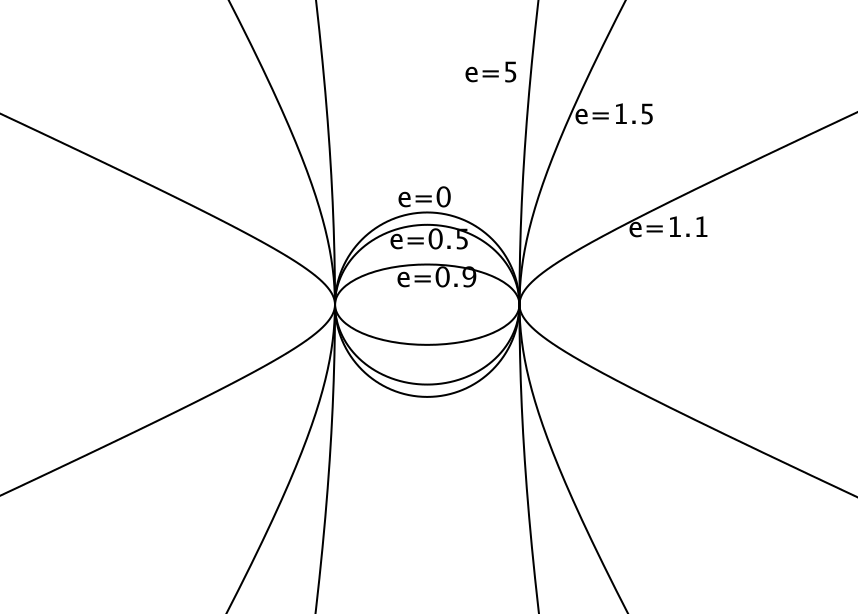
\includegraphics[width=0.75\textwidth]{img-10/excentricitats}
		\end{center}
	\end{minipage}
	 
\end{theorybox}

\begin{mylist}
	\exer[1] Calcula l'equació de la paràbola amb focus $F(3,0)$ i directriu la recta $x=-3$.
	\answers{$x=\frac{1}{12}y^2$}
	
	\exer[1] Calcula el vèrtex, focus i directriu de la paràbola $4y=(x-3)^2$.
	\answers{$V(3,0)$, $F(0, 1)$, $d: y=-1$}
	
	\exer[1] L'òrbita d'un cometa té una excentricitat $1.75$. De quina cònica es tracta? Quina és la distància més propera al focus?
	\answers{És una hipèrbola. $d=c-a=0.75 a$}
	
\end{mylist}


\pagebreak
%%%%%%%%%%%%%%%%%%%%%%%%%%%%%%%%%%%%%%%%%%%%%%%%%%%%%%%%%%%%%%%%%%%%%%%%%%%%%%%%%%%%%%%%%%%%%%%%%%%%%%%%%%%%%%%%%%%%%%%%%%%%%%%
\begin{activitats}
	
\begin{mylist}

\item  Calcula tots els elements de les el·lipses següents i dibuixa-les.
\begin{tasks} 
	\task $\dfrac{\left(x-2\right)^{2} }{3^{2} } +\dfrac{\left(y+1\right)^{2} }{4} =1$   
	\task $4x^{2} +9y^{2} -8x=0$
\end{tasks}

\answers[cols=1]{[Centre $(2,-1)$; Semieix major $a=3$; Semieix menor $b=2$; Semi-distància focal $c=\sqrt{5}$; excentricitat $e=0.745$; Focus $F'(2-\sqrt{5},-1)$ i $F'(2+\sqrt{5},-1)$; Vèrtexs $V_1(5,-1)$ \; $V_2(-1,1)$ \; $V_3(2,1)$ \; $V_4(2,-3)$,
	%%%
	Primer passam a canònica $\dfrac{(x-1)^2}{1^2}+\dfrac{y^2}{4/9}=1$\par 
	Centre $(1,0)$; Semieix major $a=1$; Semieix menor $b=2/3$; Semi-distància focal $c=\sqrt{5}/3$; excentricitat $e=0.745$; Focus $F'(1-\sqrt{5}/3,0)$ i $F'(1+\sqrt{5}/3,0)$; Vèrtexs $V_1(2,0)$ \; $V_2(0,0)$ \; $V_3(1,2/3)$ \; $V_4(1,-2/3)$]}

\item  Considera la hipèrbola $x^{2} -y^{2} +2y=0$. Calcula:
\begin{enumerate}
	\item  La seva equació canònica.
	
	\item  El seu centre i focus.
	
	\item  Les seves asímptotes. 
\end{enumerate}

\answers{[$\dfrac{(y-1)^2}{1^2}-\dfrac{x^2}{1^2}=1$,
	%%
	Es tracta d'una hipèrbola vertical (canviam els papers de $x,y$) equilàtera. Centre $(0,1)$.\par Els semieixos són $1$ i la semi-distància focal $c=\sqrt{2}$. Els focus $F(0,1+\sqrt{2})$ i $F(0,1-\sqrt{2})$.\par 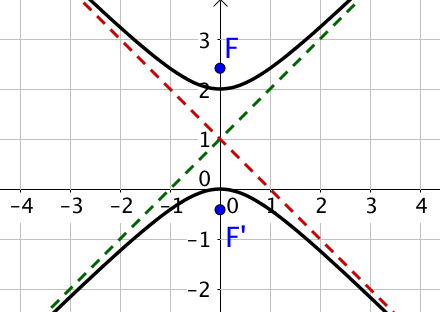
\includegraphics[width=0.4\textwidth]{img-sol/t10-13},
	%%
	Transformam l'equació com suma per diferència  $\left( (y-1) + x \right) \cdot \left( (y-1) - x \right)=1$. Les asímptotes són $y=-x+1$ i $y=x+1$
	]}


\item  Calcula tots els elements de les hipèrboles següents i dibuixa-les.
\begin{tasks} 
	\task $\left(x+1\right)^{2} -\frac{\left(y-2\right)^{2} }{4} =1$    \task  $4x^{2} -y^{2} -8x+2y=0$
\end{tasks}

\answers[cols=1]{[Centre $(-1,2)$; Semieix major $a=1$; Semieix menor $b=2$;\par Semi-distància focal $c=\sqrt{5}$; excentricitat $e=2.236$; Focus $F'(-1-\sqrt{5},2)$ i $F'(-1+\sqrt{5},2)$; Vèrtexs $V_1(0,2)$ \; $V_2(-2,2)$; Asímptotes: $y=-2x$ i $y=2x+4$ \par 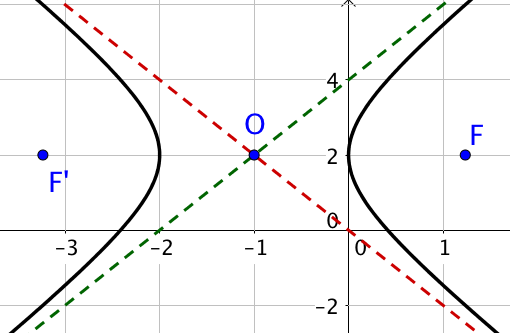
\includegraphics[width=0.4\textwidth]{img-sol/t10-14a},
	%%%
	Primer passam a canònica $\dfrac{(x-1)^2}{3/4}+\dfrac{(y-1)^2}{3}=1$\par 
	Centre $(1,1)$; Semieix major $a=\sqrt{3}/2$; Semieix menor $b=\sqrt{3}$;\par Semi-distància focal $c=\sqrt{15}/2$; excentricitat $e=2.236$; Focus $F'(1-\sqrt{15}/2,1)$ i $F'(1+\sqrt{15}/2,1)$; Vèrtexs $V_1(1+\sqrt{3}/2,1)$ \; $V_2(1-\sqrt{3}/2,1)$;\par Asímptotes: $y=-2.209x+3.309$ i $y=2.309x-1.309$ \par 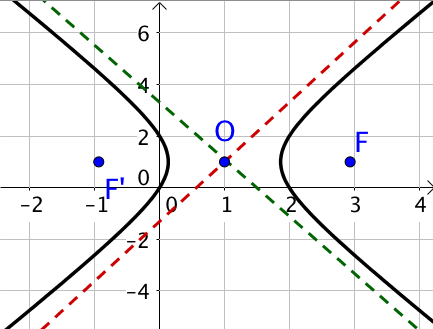
\includegraphics[width=0.4\textwidth]{img-sol/t10-14b}]}


\item  Una hipèrbola horitzontal té centre en el (1, 2) i excentricitat 2. Sabent que passa pel punt (4, 2), quina és la seva equació? [\textit{Pista}: el paràmetre \textit{a} el pots treure simplement del dibuix].

\answers{Com que $O(1,2)$ i $V(4,2)$; el semieix major $a=d(V,O)=3$. Com que $e=c/a=2$, la semi-distància focal $c=6$.\par El semieix menor $b=\sqrt{c^2-a^2}=\sqrt{27}$.\par L'equació canònica $\dfrac{(x-1)^2}{9}-\dfrac{(y-2)^2}{27}=1$.}


\item  El vèrtex d'una paràbola vertical amb les branques cap amunt és el punt (2, $-$1). Sabent que passa pel punt (1, 0) escriu l'equació de la paràbola, dibuixa-la i calcula el seu focus.

\answers{L'equació d'una paràbola vertical per amunt en centre $(2,-1)$ és de la forma $y+1=k(x-2)^2$. Substituïm el punt $(1,0)$ per trobar $k=1$.\par Aleshores, $y+1=(x-2)^2$. Sabem $\dfrac{1}{2p}=1$, per tant $p=\frac{1}{2}$. El Focus és a $F(1,-\frac{3}{4})$ i la directriu $y=-\frac{5}{4}$.\par 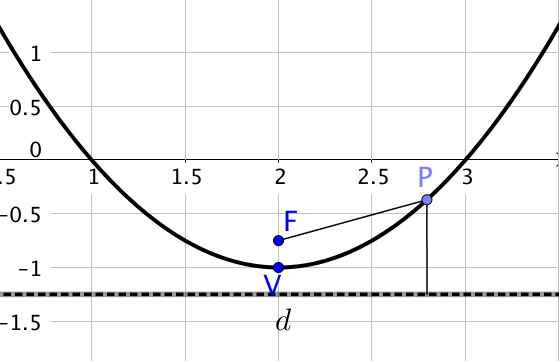
\includegraphics[width=0.4\textwidth]{img-sol/t10-16}}


\item  Identifica les figures, dibuixa-les i calcula els seus focus.
\begin{tasks} 
	\task  $2y^{2} +3x={\rm 0}$   \task  $\dfrac{\left(x+{\rm 1}\right)^{{\rm 2}} }{{\rm 9}} -\dfrac{\left(y-1\right)^2}{{\rm 4}} ={\rm 1}$     
\end{tasks}

\answers{[Canònica: $x=-\frac{1}{3/2}y^2$. Paràbola horitzontal cap a l'esquerra centrada $(0,0)$. $p=3/4$;\par El Focus $(-3/4,0)$ i la directriu $x=3/4$, 
	%%
Hipèrbola centre a $(-1,1)$ i focus $F(-1+\sqrt{13},1)$ i $F'(-1-\sqrt{13},1)$;\par Les asímptotes: $y=-\frac{2x}{3}+\frac{1}{3}$ i $y=\frac{2x}{3}+\frac{5}{3}$\par
\ggblink{https://www.geogebra.org/m/mKY89SzR}	
	]}


\begin{comment}
\item  Identifica les figures i dibuixa-les. En el cas de la hipèrbola, calcula les seves asímptotes.
\begin{tasks} 
	\task $\dfrac{\left(x+1\right)^{2} }{9} +\dfrac{\left(y-1\right)^{2} }{4} =1$   
	\task  $\dfrac{\left(x-1\right)^{2}}{16} -\dfrac{{y}^{2}}{9} =1$
\end{tasks}
\end{comment}

\item  \ggb Dibuixa amb \textit{Geogebra} o qualsevol programa equivalent les següents còniques. Classifica-les en el·lipses, paràboles o hipèrboles.
\begin{tasks} 
	\task $x^{2} +3xy=3$      \task $x^{2} +2xy+y^{2} -3y=0$   \task $x^{2} -2xy-y^{2} +4=0$
	\task $2x^{2} +4xy+y^{2} =1$  %\task $3x^{2} -6xy+y^{2} -2x=0$   %\task $4x^{2} +xy+y^{2} -2=0$
\end{tasks}

\answers{ Totes són hipèrboles obliqües excepte b) que és una paràbola també obliqua.
	\par \ggblink{https://www.geogebra.org/m/tzkCVusA}}


\item  Dibuixa les següents el·lipses i calcula els seus eixos major i menor. Series capaç de calcular la seva excentricitat? [\textit{Pista}: fes-ho amb l'ordinador, tallant l'el·lipse amb la recta focal].
\begin{enumerate}
	\item  Una el·lipse amb focus en (1, 3) i en (3, 1), que passa per l'origen.
	
	\item  Una el·lipse amb focus en ($-$1, 0) i en ($-$5, 2) que passa pel $(-1, 2)$.
\end{enumerate}	

\answers{[El centre es $O=\frac{F+F'}{2}=(2,2)$; La semidistància focal $c=dist(OF)=\sqrt{2}$; mirant el dibuix $P=(0,0)$ es troba sobre el semieix menor $b=d(PO)=2\sqrt{2}$; el semieix major $a=\sqrt{c^2+b^2}=\sqrt{10}$ excentricitat $e=0.447$
	\par \ggblink{https://www.geogebra.org/m/zf9ZxYWn},
	%%
El centre es $O=\frac{F+F'}{2}=(-3,1)$; La semidistància focal $c=dist(OF)=\sqrt{5}$; mirant el dibuix sabem que $d(F_1,P)+d(F_2,P)=2a$ es troba sobre el semieix major $a=6/2=3$; el semieix menor $b=\sqrt{a^2-c^2}=2$; excentricitat $e=0.745$
\par \ggblink{https://www.geogebra.org/m/VAX9PeVf}	
	]}


	
\item  \ggb Dibuixa, amb \textit{Geogebra} o un programa equivalent les següents hipèrboles i calcula els seus eixos major i menor. 
	\begin{enumerate}
		\item  Una hipèrbola amb focus en (1, 3) i en (3, 1) que passa pel (2, 0).
		
		\item  Una hipèrbola amb focus en $(-1, 0)$ i en $(-5, 2)$ que passa pel $(-1, 2)$.
	\end{enumerate}

\answers{\mbox{}\par \ggblink{https://www.geogebra.org/m/VJGVSq6z}}

	
\item  Dibuixa les següents paràboles i calcula el seu eix de simetria i el seu vèrtex. 
	\begin{enumerate}
		\item  Una paràbola amb focus en (1, 3) i recta directriu $y = x$.
		
		\item  Una paràbola amb focus en ($-$1, 1) i recta directriu $3x+y = 4$.
	\end{enumerate}

\answers{[
	$d(X,d)=d(X,F)$\par $(x-1)^2+(y-3)^2=\left( \dfrac{|x-y|}{\sqrt{2}} \right)^2$\par
	$x^2+y^2+2xy-4x-12y+20=0$\par
	L'eix simetria passa per focus i és perpendicular directriu $y=-x+4$,
	%%
	$d(X,d)=d(X,F)$\par $(x+1)^2+(y-1)^2=\left( \dfrac{|3x+y-4|}{\sqrt{10}} \right)^2$\par
	$x^2+9y^2-6xy+44x-12y+4=0$\par 
	L'eix simetria passa per focus i és perpendicular directriu $y=\frac{1}{3}x+\frac{4}{3}$
	\par
	\ggblink{https://www.geogebra.org/m/CxZaNSBY}
	]}

	
\item  Calcula els focus i els paràmetres \textit{a}, \textit{b} i \textit{c} de les següents hipèrboles equilàteres i dibuixa-les:
	\begin{tasks}(2)
		\task $xy=\frac{9}{2}$  \task $xy=32$   \task $xy=24$   \task $xy=1$
	\end{tasks}

\answers{\mbox{}\par 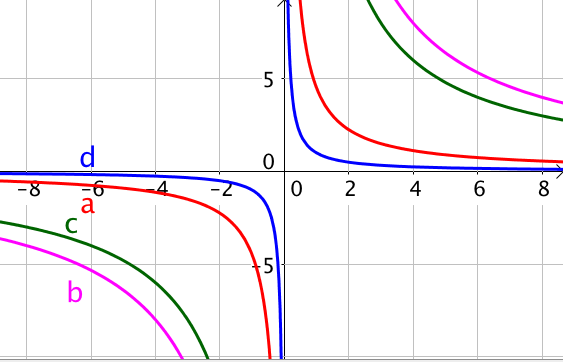
\includegraphics[width=0.4\textwidth]{img-sol/t10-22}}


\item  Identifica les figures i dibuixa-les
\begin{tasks} 
	\task   $\frac{\left(x-1\right)^{2} }{4} -\frac{\left(y+1\right)^{2} }{9} =1$   \task   $\frac{\left(x-2\right)^{2} }{3^{2} } +\frac{\left(y-1\right)^{2} }{2^{2} } =1$ \task  $y^{2} -2x=0$   
\end{tasks}

\answers{[És una hipèrbola amb centre $O(1,-1)$ i semieixos $2$ i $3$,
	És una el·lipse amb centre  $O(2,1)$ i semieixos $3$ i $2$,
	És una paràbola horitzontal cap a la dreta centrada a l'origen. El focus es  troba a $F(1/2,0)$]}
 

\item  Calculau la circumferència que passa pels punts \textit{A}=(1, 4), \textit{B}=(3, 4) i \textit{C}=(5, 5).

\answers{$x^2+y^2+Ax+By+C=0$. Plantejam i resolem un sistema $3\times 3$.\par $\left\{ \begin{array}{l}
	A+4B+C=-17\\
	3A+4B+C=-25\\
	5A+5B+C=-50
	\end{array} \right.$;\par Trobam $A=-4$; $B=-17$; $C=55$. L'equació de la circumferència és $x^2+y^2-4x-17y+55=0$. En forma canònica: $(x-2)^2+(y-\frac{17}{2})^2=\frac{85}{4}$
	\par
Solució alternativa: Calcula el circumcentre del triangle ABC.}


\item  Calculau l'equació d'una hipèrbola amb centre $O(-1, 1)$ i semi-eixos 8 i 5. Dibuixa-la.

\answers{$\dfrac{(x+1)^2}{64}-\dfrac{(y-1)^2}{25}=1$}

\item  Identifica les figures i dibuixa-les. Calcula els focus.
\begin{tasks} 
	\task  $\frac{x^{{\rm 2}} }{{\rm 4}} +y^{2} ={\rm 1}$   
	\task  $y^{2} -{\rm 2}x={\rm 1}$ 
	\task  $\frac{(x-3)^2}{9}-\frac{y^2}{4}=1$
	\task  $\frac{(x-1)^2}{4}+\frac{(y+1)^2}{9}=1$
\end{tasks}

\answers{[E·lipse centrada a l'origen; $F(\sqrt{3},0)$ i $F'(-\sqrt{3},0)$,
	Paràbola horitzontal cap a la dreta centrada a l'origen; $F(\frac{1}{2},0)$,
	Hipèrbola centrada a $(3,0)$; $F(3+\sqrt{13},0)$ i $F'(3-\sqrt{13},0)$,
	 	El·lipse vertical centrada a $(1,-1)$; $F(1,-1+\sqrt{5})$ i $F'(1,-1-\sqrt{5})$]}

\item  Identifica les figures i dibuixa-les. 
 \begin{tasks} 
 \task $x^{2} +2y^{2} -4x=0$   \task  $x^{2} -y^{2} +2y=0$ 
\end{tasks}

\answers{[Completam quadrats: $\dfrac{(x-2)^2}{4}+\dfrac{y^2}{2}=1$; és una el·lipse horitzontal en centre a $(2,0)$ i semieixos 2 i $\sqrt{2}$, 
	Completam quadrats: $-x^2 + (y-1)^2 = 1$; és una hipèrbola equilàtera vertical amb centre $(0,1)$. El seu focus es troben a $F(0,1+\sqrt{2})$ i $F'(0,1-\sqrt{2})$ 
	]}

\item  Calcula la circumferència que passa per \textit{A}=(1, 4), \textit{B} = (3, 6) i el centre de la qual és el punt mitjà de $\overline{AB}$.

\answers{$O=\frac{A+B}{2}=(2,5)$; això implica que AB és una diagonal del la circumferència. El radi és $R=d(OA)=\sqrt{2}$. L'equació: $(x-2)^2+(y-5)^2=2$ o en general $x^2+y^2-4x-10y+27=0$}

\item  Considera la hipèrbola equilàtera $xy=50$. Calcula els seus focus, excentricitat i asímptotes i dibuixa-la.
 
\begin{comment}
\item  Dibuixa amb \textit{Geogebra} o qualsevol programa equivalent les següents còniques. En funció del dibuix, classifica-les en el·lipses, paràboles o hipèrboles.

 \begin{tasks} 
	\task  $x^{2} -3xy=2$  \task $x^{2} +xy+y^{2} -y=0$  \task $2x^{2} -4xy+y^{2} +4=0$
	\task  $x^{2} -2xy+2y^{2} =1$   \task $3x^{2} -6xy+4y^{2} -2x=0$  \task $4x^{2} +xy+y^{2} -2=0$
\end{tasks}
\end{comment}

\item  Una el·lipse té focus en (1, 1) i en (4, 1) i passa pel punt (0, 1). Calcula la seva equació i dibuixa-la. Quant val la seva excentricitat?

\answers{Centre $O(5/2,1)$; $c=3/2$; $a=5/2$; $b=2$; $\dfrac{(x-5/2)^2}{25/4}+\dfrac{(y-1)^2}{4}=1$; $e=3/5=0.6$}

\item  Una el·lipse té centre al punt (1, $-$1) i passa pels punts (5, $-$1) i (1, 1). Sabent que el semi-eix major és 4, a) Dóna la seva equació i dibuixa l'el·lipse, b) Calcula els seus focus i l'excentricitat.  

\answers{Dels dos punts que ens donen deduïm els semieixos major 4 i menor 2. L'equació és $\dfrac{(x-1)^2}{16}+\dfrac{(y+1)^2}{4}=1$, $c=\sqrt{4^2-2^2}=2\sqrt{3}$; Focus a $F(1+2\sqrt{3},-1)$ i $F(1-2\sqrt{3},-1)$; excentricitat $e=\frac{\sqrt{3}}{2}=0.866$} 

\item  Una hipèrbola equilàtera amb centre a l'origen i passa pel punt (1, 3). Calcula els seus focus i dibuixa-la.

\answers{Si és equilàtera horitzontal i centrada a l'origen, serà de la forma $x^2-y^2=a^2$. Substituint el punt $1^2-3^2=a^2$, això no és possible.\par Aleshores, la hipèrbola ha d'ésser vertical $-x^2+y^2=8$. essent $a=b=2\sqrt{2}$; $c=4$ i els focus són als punts $F(0,4)$ i $F'(0,-4)$}

\item  Sabent que les asímptotes d'una hipèrbola són $y=2x$ i $y=-2x$ i que passa pel punt (2,0), calcula la seva equació.

\answers{Com que les asímptotes es tallen al (0,0) aquest és el centre de la hipèbola. És a dir, està centrada a l'origen. $y=\pm \frac{b}{a}x$; aleshores sabem que $b=2a$. L'equació és $\dfrac{x^2}{a^2}-\frac{y^2}{4a^2}=1$. Si hi substituïm el punt (2,0) trobam que $a=\sqrt{2}$ i $b=2\sqrt{2}$.\par 
	L'equació és $\dfrac{x^2}{2}-\frac{y^2}{8}=1$}

\item  Una hipèrbola equilàtera té com a equació $xy=8$. Calcula els seus focus. 

\answers{En general $x\cdot y=k$ amb $k>0$; tindrà els vèrtex sobre la recta $y=x$ i seran $V(\pm \sqrt{k}, \pm \sqrt{k})$. El semieix major per Pitàgores $a=\sqrt{2k}$. Com que és equilàtera $a=b=\sqrt{2k}$. \par
Trobam la semi-distància $c=\sqrt{a^2+b^2}=2\sqrt{k}$ sobre la recta $y=x$, per trigonometria podem localitzar els vèrtexs (projectam l'angle de $45^\circ$) $F(\sqrt{k},\sqrt{k})$ i $F(-\sqrt{2k},-\sqrt{2k})$.
\par 
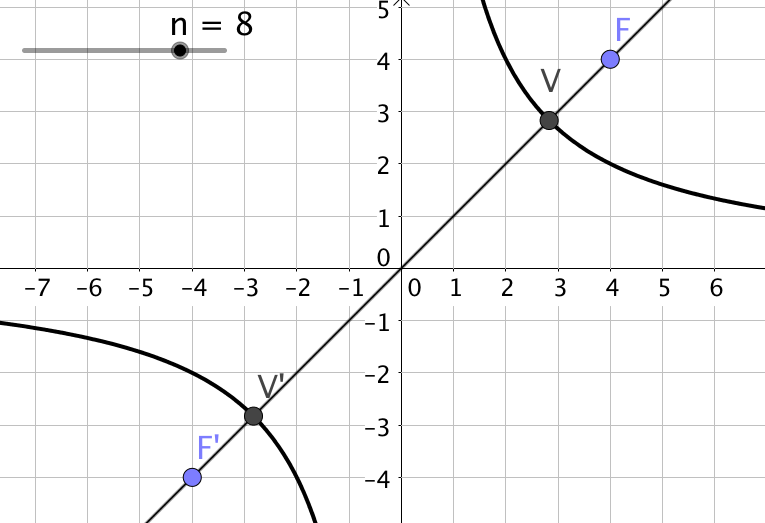
\includegraphics[width=0.4\textwidth]{img-sol/t10-34}
\par
Pel nostre cas $k=8$ i els focus són a $F(4,4)$ i $F(-4,-4)$.
}
\end{mylist}


\end{activitats}

\begin{autoaval}{22}

\begin{mylist}
	\exer[2]  Calcula l'equació de la circumferència que passa pels punts $P(4,5)$, $Q(-3,4)$ i $R=(6,1)$. Suposa que l'equació és de la forma $x^2+y^2+Ax+By+C=0$ i planteja un sistema d'equacions per trobar $A$, $B$ i $C$.
	\answers{$x^2+y^2-2x-2y-23=0$ o $(x-1)^2+(y-1)^2=25$. Té centre $O(1,1)$ i radi $R=5$.}
	
	\exer[2] Calcula l'equació de l'el·lipse horitzontal amb centre en $O(-1,3)$ i semi-eixos 5 i 3. Calcula els seus focus i dibuixa-la. Què val l'excentricitat?
	\answers{$\frac{(x+1)^2}{25}+\frac{(y-3)^2}{9}=1$. La semi-distància focal $c=4$, els focus són $F'(-5,3)$ i $F(3,3)$, i l'excentricitat $e=0.8$.}
		
	\exer[2] Dibuixa la hipèrbola $x^2-2y^2=4$ i les seves asímptotes. Calcula els seus focus i l'excentricitat.
	\answers{Semi-eixos: $a=2$, $b=\sqrt{2}$, les asímptotes $y=\pm\frac{\sqrt{2}}{2}x$, semi-distància focal: $c=\sqrt{6}$ i l'excentricitat $e=1.225$.}
	
	\exer[2] Una paràbola vertical té el vèrtex en $V(1,2)$ i les branques cap amunt. Si sabem que passa pel punt $P(0,5)$, calcula la seva equació, l'equació de la directriu i la posició del focus.
	\answers{La distància focus-directriu és $p=1/6$, l'equació $y-2=3 (x-1)^2$, la directriu és la recta $y=23/12$ i la posició del focus $F(1, 25/12)$.}
	
	\exer[2] Identifica les còniques i dibuixa-les:
	  \begin{tasks}(3)
	  		\task $\frac{(x-1)^2}{4}+y^2=1$	
	  		\task $x^2-2x+y^2-4y+1=0$
	  		\task $x^2-3y=6$
	  \end{tasks}
	\answers{a) El·lipse de centre $(1,0)$ i semi-eixos $a=2$, $b=1$.  b) Circumferència de centre $(1,2)$ i radi $2$. c) Paràbola vertical de vèrtex $(0,-2)$ i distància Focus-directriu $p=3/2$.}
\end{mylist}
\end{autoaval}